\subsection{Aspects of Software Development}
  \begin{figure}[H]
    \centering
    \begin{tikzpicture}
      \def \n {5}
      \def \radius {5cm}
      \def \margin {10} % margin in angles, depends on the radius
      \def\names{{"", "Analysis", "Design", "Implementation", "Testing", "Evaluation"}}
      \foreach \s in {1,...,\n}
      {
        \node at ({180-(360/\n * (\s - 0)+18)}:\radius) {\pgfmathparse{\names[\s]}\pgfmathresult};
        \draw[<-, >=latex] ({360/\n * (\s - 1)+\margin+18}:\radius)
        arc ({360/\n * (\s - 1)+\margin+18}:{360/\n * (\s)-\margin+18}:\radius);
      }
    \end{tikzpicture}
  \end{figure}
  \noindent
  \marginnote{3.3.1.1}Analysis is first stage of system development cycle where the problem is initially identified (through understanding what has promted the need for a new computer system) and researched(through gathering information and feasibility study).\\
  During this stage the problem you will need to try and define the actual problems that will need to be solved, and try to be realistic with the resources available, a list of constraining factors may be identified, to obtain a feasible solution. A specification and discussion of the scope of the work should be done if you are working for someone else.\\
  There are several reasons why a company may want a new computer system, some of the reasons are:
  \begin{itemize}
    \setlength\itemsep{0cm}
    \item The existing system is not capable of handling the increasing volume of data being required.
    \item New technology means the old system is obsolete.
    \item The current system may be inflexible or inefficient.
    \item New technology has created new opportunities for expansion/ creation of systems.
    \item Commercial Reasons, Improved to generate increased demand of the system.
    \item Develop systems for a new platform or Operating System.
    \item To take advantage of increased processing and network power
  \end{itemize}
  If you are analysing an existing system, then you should aim to gather information about the current system, this can be done in many ways such as:
  \begin{itemize}
    \setlength\itemsep{0em}
    \item Interview people who are involved with the current system.
      \subitem This can be quite time consuming but allows you to easily obtain in-depth information about the system, although this information will be somewhat subjective.
    \item Asking people currently involved with the system to answer a questionnaire or survey.
      \subitem Questionnaires allow for quick data gathering, however they often only allow limited information to be gathered as if you want easily analysable data, you will have to use closed questions.
    \item Observation of current practices when interacting with the system.
      \subitem Although this can be very time consuming, it is more objective rather than subjective and can lead to spotting something others did not.
    \item Examination of the current system files, paperwork and processes.
      \subitem This will help to inform you of the data requirements of the new system, how to develop the human-controller interface (HCI), and the overall scope of the problem.
  \end{itemize}
  A feasibility study is an analysis of whether it is possible or desirable to create a system. The report will indicate how practical a solution may be in terms of many factors such as time, availability of software and hardware, and UI.\\
  \marginnote{3.3.1.2} Design is the second stage of the system development cycle and is where the algorithms, data and interface are designed.\\
  On big projects it is often difficult to consider the problem as a one problem, so the problem is broken down into smaller units, which can then themselves be broken down further, this is known as top-down design. This is similar to modular design where the main problem is broken down into several self-contained modules. Both approaches allow multiple programmers to work on the solution, and both require a defined feel so that the different parts of the program flow together. The main risk with Top-down design is that a person may get too invested in a specific detail without having completed the overall section fo the program.\\
  Data Flow Diagrams are a visual method of showing how data passes around a system, it only requires 4 symbols:
  \begin{center}
    \begin{tabular}{ m{3cm} m{3cm} m{3cm} m{3cm} }
      Entity & Process & Storage & Data flow \\
      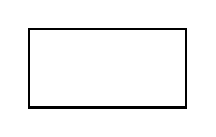
\begin{tikzpicture}
        \draw[thick] (0,0) rectangle (2,1);
      \end{tikzpicture}
      &
      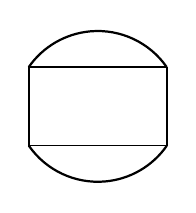
\begin{tikzpicture}
        \draw (0,0) rectangle (1.75,1);
        \draw[thick] (0,0) -- (0,1);
        \draw[thick] (1.75,0) -- (1.75,1);
        \draw[thick] (0,0) arc (214.85:325.15:1.067cm);
        \draw[thick] (1.75,1) arc (34.85:145.15:1.067cm);
      \end{tikzpicture}
      &
      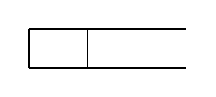
\begin{tikzpicture}
        \draw[thick] (0,0) -- (2,0);
        \draw[thick] (0,0.5) -- (2,0.5);
        \draw[thick] (0,0) -- (0,0.5);
        \draw (0.75,0) -- (0.75,0.5);
      \end{tikzpicture}
      &
      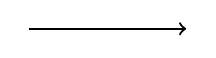
\begin{tikzpicture}
        \draw[thick,->] (0,0) -- (2,0);
      \end{tikzpicture}
      \\
    \end{tabular}
  \end{center}
  During the design phase, you may want to identify and describe the algorithms to be used within the system. It may be appropriate to write the algorithms in pseudo-code that reflects the programming paradigm being used.\\
  A data dictionary is a list of all the data being used in the system including its name, length, name, data type and validation. This should be used only when relevant (mainly in databases).\\
  A variable table is a list of all the variables that a program will use, including names, scope and data types. this is useful as it allows the programmer to have tighter control of the program being made. At this stage, names of subroutines can also be identified and the type of data to be returned.\\
  When building a system, the volumetrics of the system should be considered. The volumetrics of a system is the amount of data the system has to deal with in a given time span. Larger volumetrics implies a different way of handling data, leaning towards mass optimisation of a system. Volumetrics are very important when dealing with databases and the realisation needs to be made that the databases we have seen (e.g School Registers) are microscopic when compared to databases with over 20 million members and 100s of fields (e.g DVLA database).\\
  The human-computer interface is the term given to any form of interaction between a computer and its user. Factors to consider are:
  \begin{itemize}
    \setlength\itemsep{0em}
    \item Ease of Use: The user should be able to use the system reasonably easily.
    \item Target Audience: The age and personality of the user will directly impact how they will use the system.
    \item Technology: The technology the user uses will directly impact the features and limits of the system being developed.
    \item Ergonomics: The comfortability of the system should be taken into high regard.
  \end{itemize}
  \marginnote{3.3.1.3}Implementation is the third stage of the system development cycle and is where the actual code and data structures are created. Just to note, not all of the program needs to be written at once for example, one module may be being implemented while others are being designed.\\
  A prototype is a stripped down version of a whole system built at the design stage to test whether the concept works. At this stage the end user is asked to comment on the product so far, and they will check to make sure all the major functions work as expected.\\
  \marginnote{3.3.1.4}Testing is the fourth stage of the system development cycle and is where a range of tests are performed on the program using a variety of data. There are three different types of data that is used once each module has been completed. These are:
  \begin{itemize}
    \setlength\itemsep{0em}
    \item Normal
      \subitem This is data that the system is expected handle without issue.
    \item Boundary
      \subitem This is data that is on the extremes of the acceptable values.
    \item Erroneous.
      \subitem This is data that is clearly incorrect and expect the program to catch the error.
  \end{itemize}
  During Development several different tests are done on the modules, these test are:
  \begin{itemize}
    \setlength\itemsep{0em}
    \item Black Box Testing
      \subitem This test checks whether a specific input causes the expected output, without seeing how it is actually done.
    \item White Box Testing
      \subitem This test checks all pathways through the code, looking inside it and potentially adding extra commands to check what is happening.
    \item Unit Testing
    \subitem This checks that each unit/ module/component is fully functional by itself. It uses both white and black testing.
  \end{itemize}
  Once all the units have been tested and are fully functional, the units are first put together to create large modules and  undergo integration testing, and checks whether the different modules made from individual units, will work together. Once integration testing is complete, the program then undergoes system testing as one large single unit. System testing involves a range of tests to be carried out on the system to check whether the system satisfies the specification set out in the analysis stage. The main parts of system testing are:
  \begin{itemize}
    \setlength\itemsep{0em}
    \item Alpha Testing
      \subitem this is done in-house once the system is complete and tries to simulate possible eventualities of the system under normal conditions. The benefits are it allows the program to be corrected before the full system is released, and the original set of data is known and can thus be more easily analysed.
    \item Beta Testing
      \subitem This occurs after alpha and is when the system is given to users, who are expected to give feedback about bugs, so that the programmers can resolve them. The benefits of this is that due to the fact it has been given to people who have never used the system, they may use it in different ways and therefore highlight problems they may not have been seen in alpha testing.
    \item Acceptance Testing
      \subitem This is where the intended user test the system by entering their own data and making sure the system matches the specification that was agreed with the program writers.
  \end{itemize}
  \marginnote{3.3.1.5}Evaluation is the final stage of system development where the system is judged according to certain criteria (i.e. The specification set in the Analysis stage) and improvements are suggested. There may be several criteria used to evaluate a system, e.g:
  \begin{itemize}
    \setlength{\itemsep}{0em}
    \item Functionality
    \item Ease of Use
    \item Ease of Implementation (How easy is it to go from old system to new system)
    \item Reliability
    \item Performance
    \item Cost Effectiveness
    \item Ease of Maintenance and Adaptability
    \item Longevity
  \end{itemize}
